\section{Вычислительные эксперименты}

    \subsection{Алгоритм}
        Для реализации моделей сделаем замену переменных \( u(t) = \dot{x}(t), \quad v(t) = \dot{y}(t) \), и получим систему дифференциальных уравнений первого порядка:
        \[
            \left\{\begin{split}
                & \dot{x} = u, & \dot{y} = v, \\
                & \dot{u} = 2 \Omega v, & \dot{v} = -2 \Omega u, \\
                & x(0) = x_0, & y(0) = y_0, \\
                & u(0) = x_1, & v(0) = y_1.
            \end{split}\right.
        \]

        Для компьютерного вычисления будем использовать метод Рунге-Кутты, с помощью которого получим численное решение системы дифференциальных уравнений с заданными параметрами. После чего построим их решения и фазовые плоскости.

        По полученному закону сохранения энергии можем вывести соотношение: \( u^2 + v^2 - x_1^2 - y_1^2 = 0 \). Также проверим его выполнение для численного решения.



    \subsection{Программа}
        Для расчётов и визуализации был использован язык Python с библиотеками numpy и matplotlib.

    \subsection{Результаты}
        Построим траектории, выходящие из точки \( (5, 3) \) и имеющие начальные скорости: \( (4, 4), (5, 5), (1, 1), (-3, 3), (-4, -2), (1, -3) \) на отрезке времени \( [0, 5] \). Также покажем закон сохранения энергии.

        Для начала возьмём \( \Omega = 1 \).
        \begin{figure}[H]
            \centering
            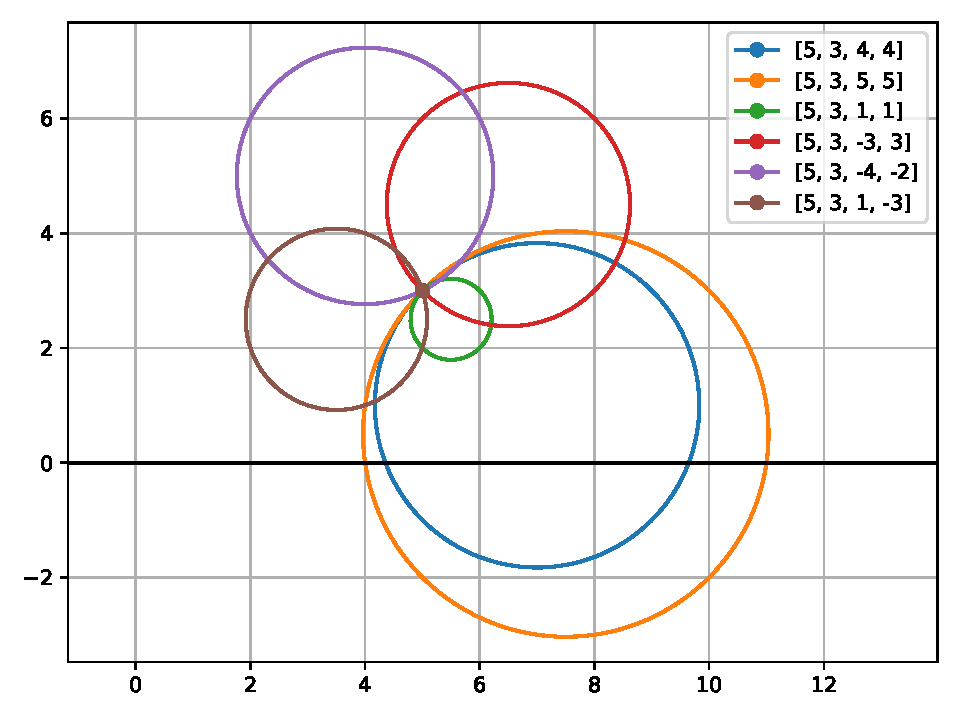
\includegraphics[width=8cm]{pictures/n1e5plot.pdf}
            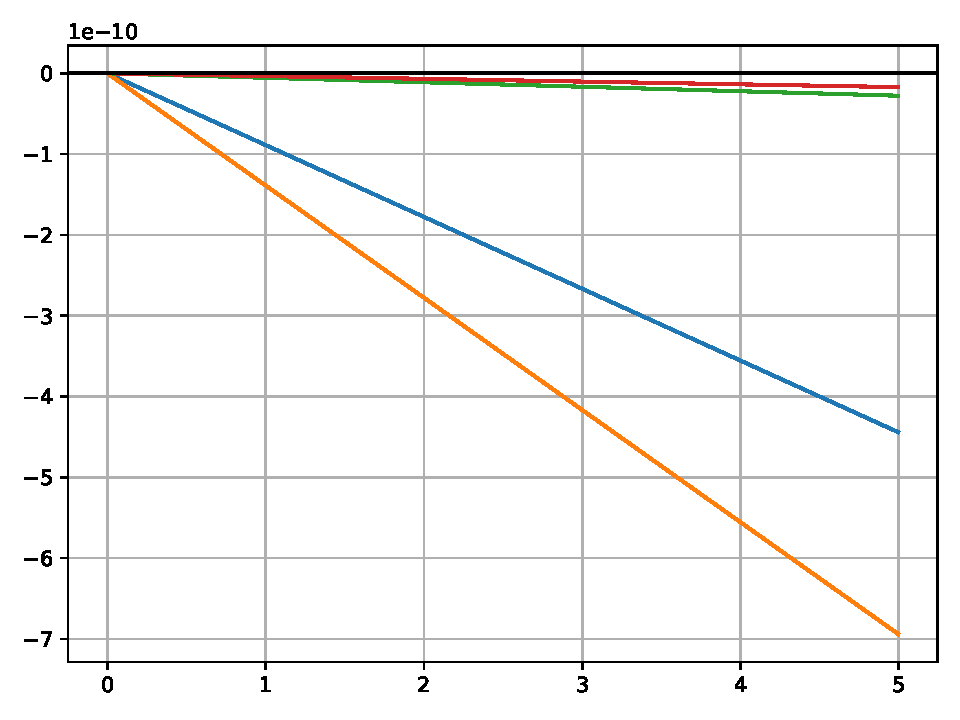
\includegraphics[width=8cm]{pictures/n1e3conv.pdf}
            \caption{Результат при количестве разбиений отрезка \( n = 1000 \).}
        \end{figure}

        \begin{figure}[H]
            \centering
            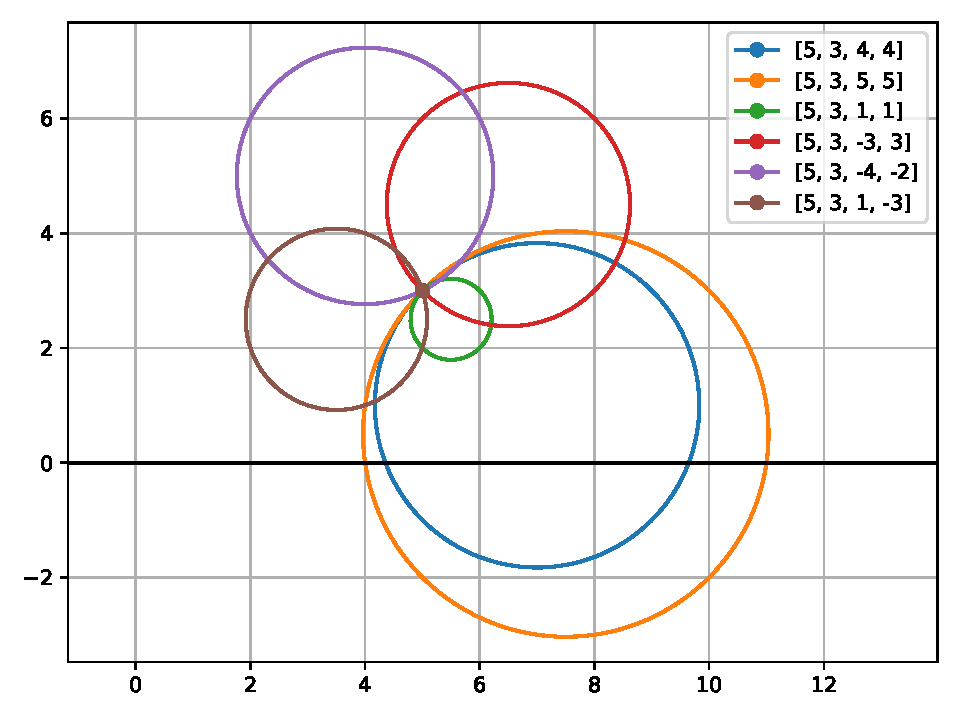
\includegraphics[width=8cm]{pictures/n1e5plot.pdf}
            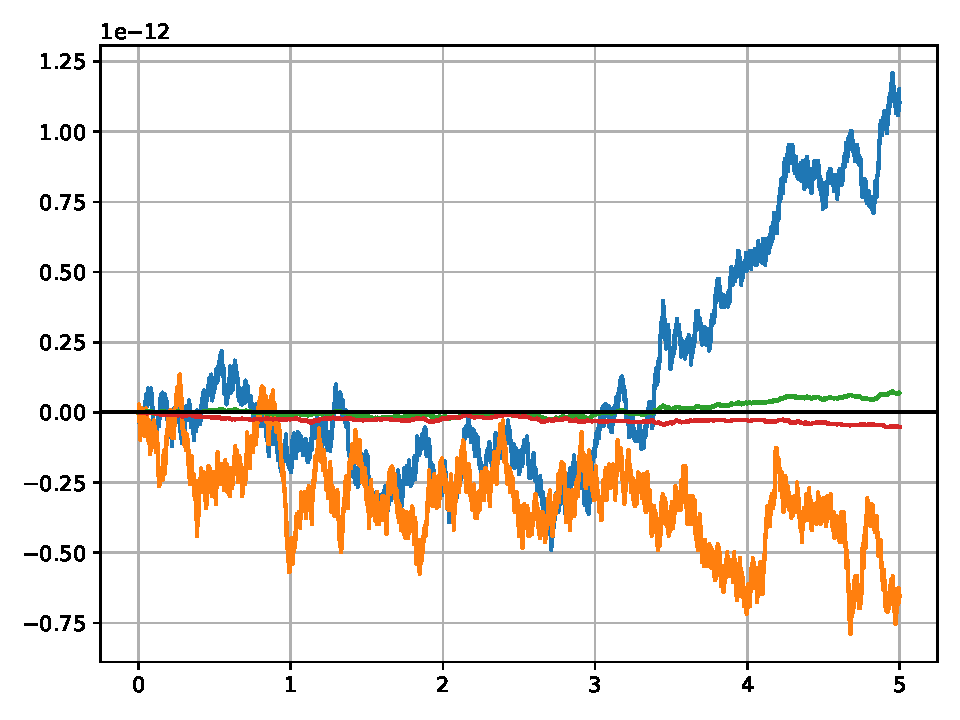
\includegraphics[width=8cm]{pictures/n1e5conv.pdf}
            \caption{Результат при количестве разбиений отрезка \( n = 100000 \).}
        \end{figure}

        Из графиков движения видно, что траекторией тела, которое находится во вращающейся системе координат, является окружность. Видно, что чем больше начальная энергия \( (u^2 + v^2) \), тем больше радиус окружности у траектории.

        У первого эксперимента с малым количеством разбиений отрезка времени погрешность относительно большая, из-за чего закон сохранения энергии не выполняется. У второго же, точно больше и можно сказать, что соотношение выполняется с некоторой погрешностью. Также из обоих экспериментов видно, что чем меньше радиус, тем меньше и погрешность в сохранении энергии.

        Теперь возьмём \( \Omega = 10 \).
        \begin{figure}[H]
            \centering
            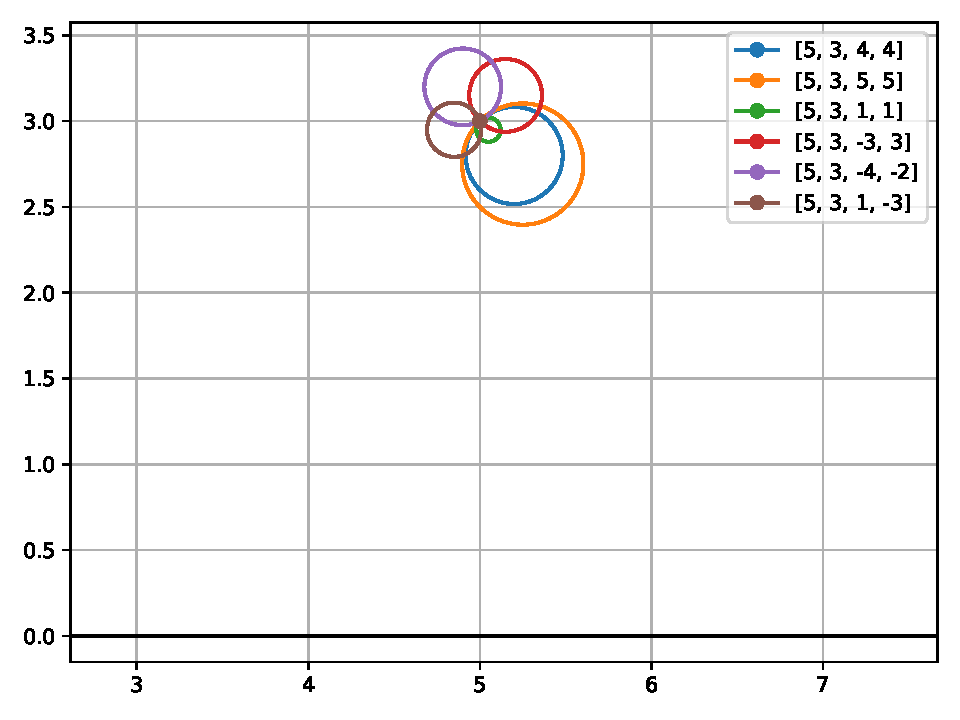
\includegraphics[width=10cm]{pictures/n1e5plot2.pdf}
            \caption{Траектории при \( \Omega = 10 \).}
        \end{figure}

        \begin{figure}[H]
            \centering
            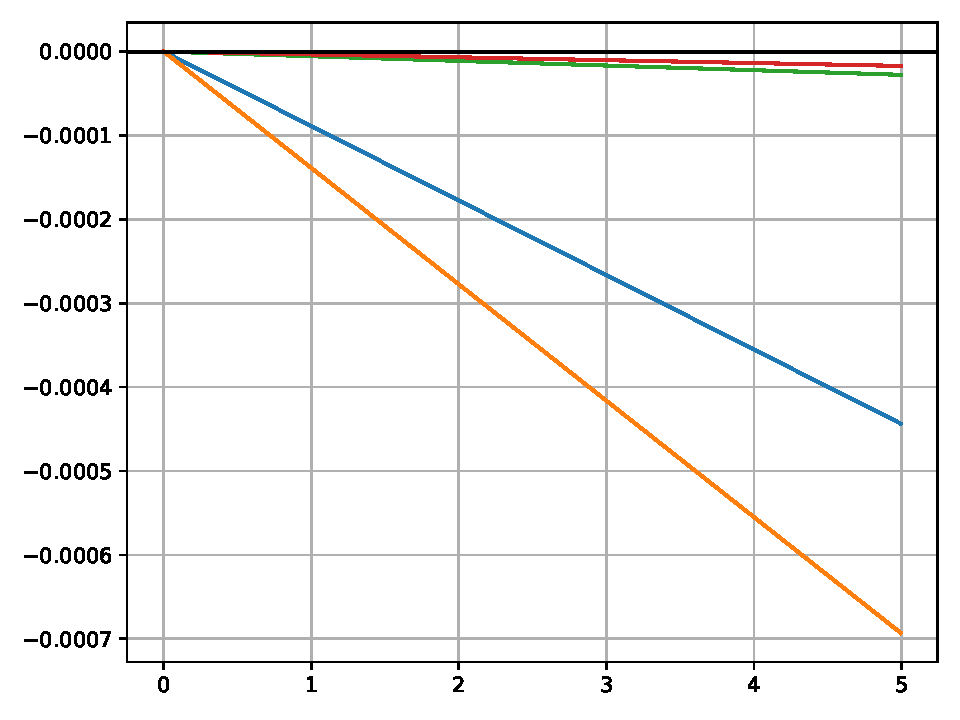
\includegraphics[width=8cm]{pictures/n1e3conv2.pdf}
            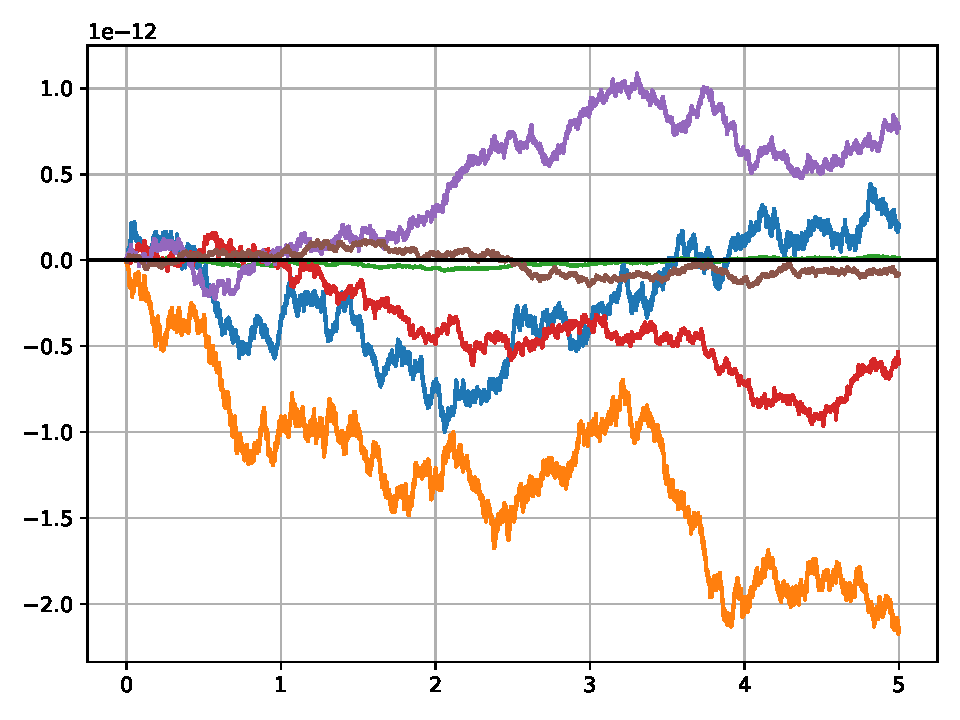
\includegraphics[width=8cm]{pictures/n1e5conv2.pdf}
            \caption{Закон сохранения при количестве \( n = 1000 \) и \( n = 100000 \).}
        \end{figure}

        При большей угловой скорости вращения получаем окружности меньшего радиуса. Аналогично ведут себя результаты, показывающие закон сохранения энергии.
